\documentclass[12pt,a4paper]{article}
\usepackage[margin=1.5cm]{geometry}
\usepackage[T1]{fontenc}
\usepackage[utf8]{inputenc}
\usepackage{lmodern}
\usepackage{booktabs}
\usepackage{tabularx}
\usepackage{array}
\usepackage{enumitem}
\usepackage{xcolor}
\usepackage{hyperref}
\usepackage{microtype}
\usepackage{tikz}
\usetikzlibrary{shapes.geometric, arrows.meta, positioning, calc, fit, backgrounds, decorations.pathreplacing}

\definecolor{brand}{HTML}{176B52}
\definecolor{brandlight}{HTML}{E8F4F0}
\definecolor{branddark}{HTML}{0E4D3B}
\definecolor{muted}{HTML}{5F716B}
\definecolor{warningbg}{HTML}{FFFBEB}
\definecolor{alertred}{HTML}{B91C1C}

\hypersetup{colorlinks=true,linkcolor=brand,urlcolor=brand,citecolor=brand}
\setlength{\parindent}{0pt}
\setlength{\parskip}{0.55em}

\tikzset{
  umlclass/.style = {rectangle, draw=branddark, fill=white, minimum width=3.4cm, text width=3.2cm, inner sep=0.2cm, font=\scriptsize},
  umlheader/.style = {rectangle, draw=branddark, fill=brandlight, minimum width=3.4cm, text width=3.2cm, inner sep=0.15cm, text centered, font=\scriptsize\bfseries},
  layerbox/.style = {rectangle, rounded corners=3pt, draw=brand, fill=brandlight, minimum width=15cm, minimum height=1.3cm, text width=14.6cm, inner sep=0.25cm, font=\footnotesize},
  flowarrow/.style = {thick, -{Stealth[length=2.2mm]}, draw=brand},
  dashedarrow/.style = {thick, dashed, -{Stealth[length=2.2mm]}, draw=muted}
}

\title{\textbf{Technical Design and Evaluation Plan Specification}\\[0.4em]
  \large COMP2300 Deliverable 3 Companion Specification\\
  \normalsize Architectural Blueprints, UML Models, Sprint Slices, and Evaluation Protocol}
\author{Arnav Mishra \and Keshav Singhal \and Hiranya Makkar\\[0.4em]
  \small Department of Electronics and Computer Science, University of Southampton}
\date{November 2026}

\begin{document}
\maketitle

\section{System Architecture Overview}
The Footprint Lens system separates graphical presentation from domain rules and local storage to guarantee that all calculations and constraint rules are testable without a GUI harness.

\begin{figure}[ht]
\centering
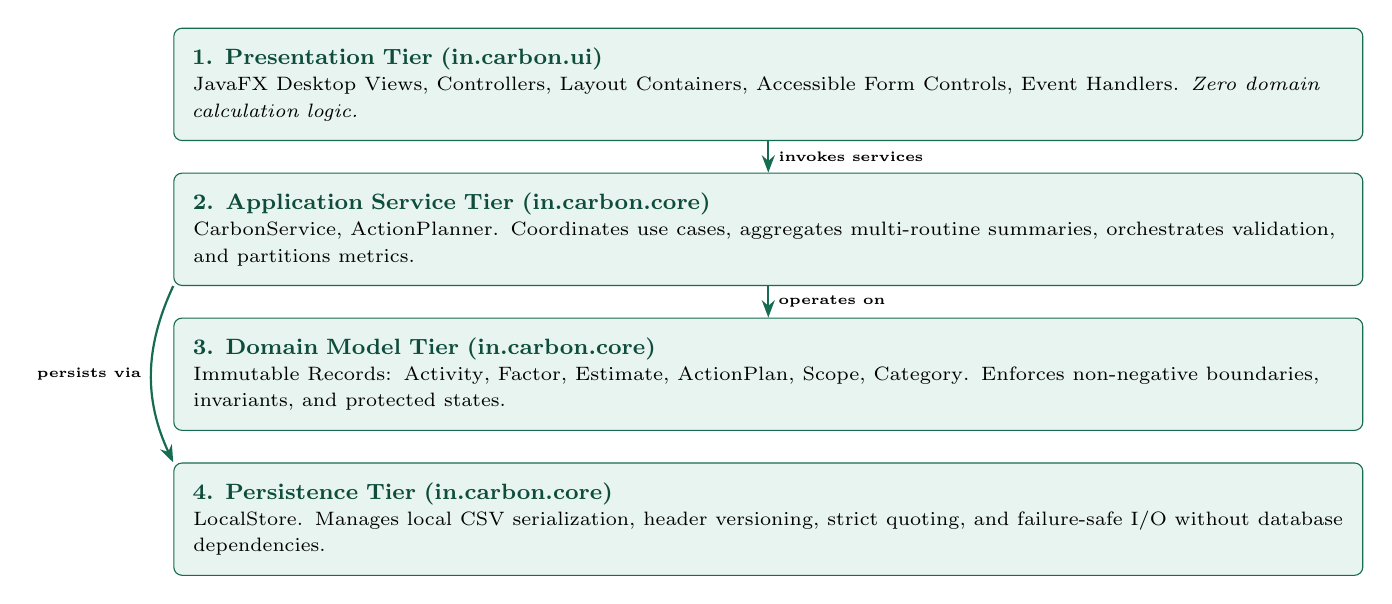
\begin{tikzpicture}[node distance=0.5cm]
  \node[layerbox] (ui) {
    \textbf{\color{branddark}1. Presentation Tier (\code{in.carbon.ui})}\\
    \scriptsize JavaFX Desktop Views, Controllers, Layout Containers, Accessible Form Controls, Event Handlers. \emph{Zero domain calculation logic.}
  };
  \node[layerbox, below=0.4cm of ui] (app) {
    \textbf{\color{branddark}2. Application Service Tier (\code{in.carbon.core})}\\
    \scriptsize \code{CarbonService}, \code{ActionPlanner}. Coordinates use cases, aggregates multi-routine summaries, orchestrates validation, and partitions metrics.
  };
  \node[layerbox, below=0.4cm of app] (domain) {
    \textbf{\color{branddark}3. Domain Model Tier (\code{in.carbon.core})}\\
    \scriptsize Immutable Records: \code{Activity}, \code{Factor}, \code{Estimate}, \code{ActionPlan}, \code{Scope}, \code{Category}. Enforces non-negative boundaries, invariants, and protected states.
  };
  \node[layerbox, below=0.4cm of domain] (persist) {
    \textbf{\color{branddark}4. Persistence Tier (\code{in.carbon.core})}\\
    \scriptsize \code{LocalStore}. Manages local CSV serialization, header versioning, strict quoting, and failure-safe I/O without database dependencies.
  };

  \draw[flowarrow] (ui) -- node[right, font=\tiny\bfseries] {invokes services} (app);
  \draw[flowarrow] (app) -- node[right, font=\tiny\bfseries] {operates on} (domain);
  \draw[flowarrow] (app.south west) to[bend right=25] node[left, font=\tiny\bfseries] {persists via} (persist.north west);
\end{tikzpicture}
\caption{Tiered Layered Clean Architecture}
\end{figure}

\section{UML Class Model}

\begin{figure}[ht]
\centering
\begin{tikzpicture}[node distance=0.8cm and 0.6cm]
  \node[umlheader] (cshead) {CarbonService};
  \node[umlclass, below=0cm of cshead] (csbody) {
    + estimate(Activity): Estimate\\
    + totalsByMetric(List): Map\\
    + waterBuckets(BigDecimal): BigDecimal
  };
  \node[fit={(cshead)(csbody)}, inner sep=0pt] (cs) {};

  \node[umlheader, right=1.0cm of cshead] (aphead) {ActionPlanner};
  \node[umlclass, below=0cm of aphead] (apbody) {
    + suggestion(Activity): Optional\\
    - isEligible(Activity, Rule): boolean
  };
  \node[fit={(aphead)(apbody)}, inner sep=0pt] (ap) {};

  \node[umlheader, below=1.2cm of csbody] (acthead) {Activity \guillemotleft record\guillemotright};
  \node[umlclass, below=0cm of acthead] (actbody) {
    - id: String\\
    - category: Category\\
    - quantity: BigDecimal\\
    - scope: Scope\\
    - protectedChoice: boolean\\
    - factor: Factor\\
    + estimate(): Estimate\\
    + displayName(): String
  };
  \node[fit={(acthead)(actbody)}, inner sep=0pt] (act) {};

  \node[umlheader, right=1.0cm of acthead] (facthead) {Factor \guillemotleft record\guillemotright};
  \node[umlclass, below=0cm of facthead] (factbody) {
    - value: BigDecimal\\
    - denominatorUnit: String\\
    - metric: String\\
    - source: String\\
    - year: String\\
    - status: FactorStatus\\
    + summary(): String
  };
  \node[fit={(facthead)(factbody)}, inner sep=0pt] (fact) {};

  \node[umlheader, below=1.2cm of actbody] (esthead) {Estimate \guillemotleft record\guillemotright};
  \node[umlclass, below=0cm of esthead] (estbody) {
    - available: boolean\\
    - value: BigDecimal\\
    - metric: String\\
    - explanation: String\\
    + numeric(...): Estimate\\
    + unavailable(...): Estimate
  };
  \node[fit={(esthead)(estbody)}, inner sep=0pt] (est) {};

  \node[umlheader, right=1.0cm of esthead] (storehead) {LocalStore};
  \node[umlclass, below=0cm of storehead] (storebody) {
    - path: Path\\
    + save(List$<$Activity$>$): void\\
    + load(): List$<$Activity$>$\\
    - formatCsv(Activity): String
  };
  \node[fit={(storehead)(storebody)}, inner sep=0pt] (store) {};

  \draw[flowarrow] (cs) -- (act);
  \draw[flowarrow] (ap) -- (act);
  \draw[flowarrow] (act) -- (fact);
  \draw[flowarrow] (act) -- (est);
  \draw[flowarrow] (store) -- (act);
\end{tikzpicture}
\caption{UML Class Diagram for Footprint Lens Core Domain}
\end{figure}

\section{UML Sequence Trace: Activity Logging and Provenance Evaluation}

\begin{figure}[ht]
\centering
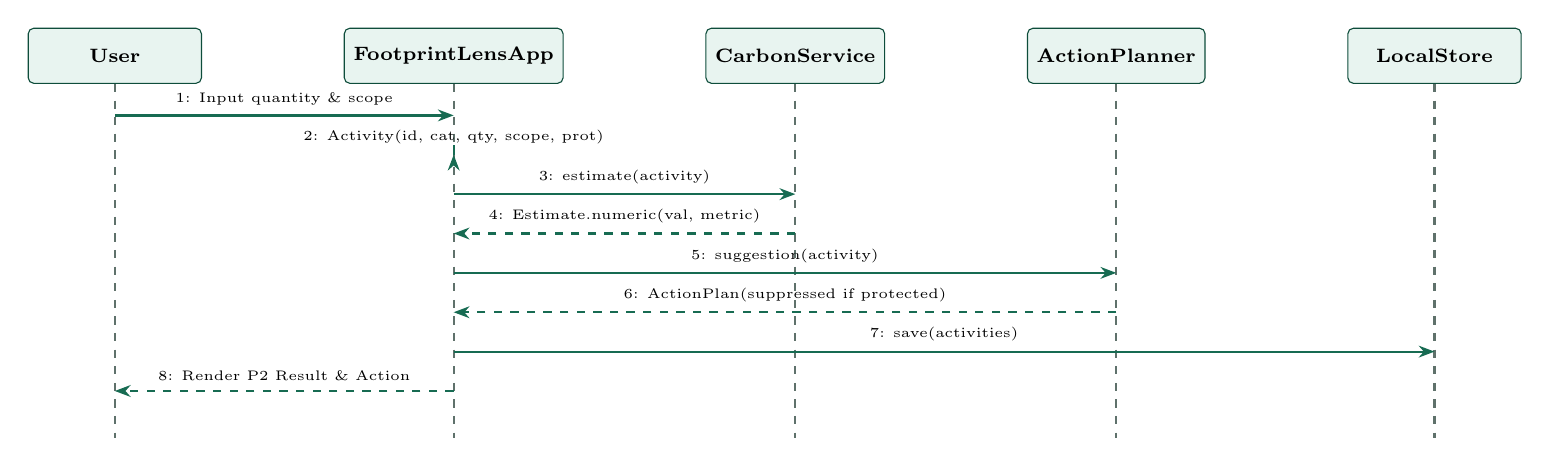
\begin{tikzpicture}[
  lifeline/.style = {dashed, draw=muted, thick},
  entity/.style = {rectangle, rounded corners=2pt, draw=branddark, fill=brandlight, minimum width=2.2cm, minimum height=0.7cm, text centered, font=\scriptsize\bfseries},
  call/.style = {thick, -{Stealth[length=2mm]}, draw=brand},
  ret/.style = {thick, dashed, -{Stealth[length=2mm]}, draw=brand}
]
  \node[entity] (u) {User};
  \node[entity, right=1.8cm of u] (ui) {FootprintLensApp};
  \node[entity, right=1.8cm of ui] (cs) {CarbonService};
  \node[entity, right=1.8cm of cs] (ap) {ActionPlanner};
  \node[entity, right=1.8cm of ap] (ls) {LocalStore};

  \coordinate (u_b) at ($(u.south) + (0, -4.5)$);
  \coordinate (ui_b) at ($(ui.south) + (0, -4.5)$);
  \coordinate (cs_b) at ($(cs.south) + (0, -4.5)$);
  \coordinate (ap_b) at ($(ap.south) + (0, -4.5)$);
  \coordinate (ls_b) at ($(ls.south) + (0, -4.5)$);

  \draw[lifeline] (u) -- (u_b);
  \draw[lifeline] (ui) -- (ui_b);
  \draw[lifeline] (cs) -- (cs_b);
  \draw[lifeline] (ap) -- (ap_b);
  \draw[lifeline] (ls) -- (ls_b);

  \draw[call] ($(u.south)+(0,-0.4)$) -- node[above, font=\tiny] {1: Input quantity \& scope} ($(ui.south)+(0,-0.4)$);
  \draw[call] ($(ui.south)+(0,-0.9)$) -- node[above, font=\tiny] {2: Activity(id, cat, qty, scope, prot)} ($(ui.south)+(0,-0.9)$);
  \draw[call] ($(ui.south)+(0,-1.4)$) -- node[above, font=\tiny] {3: estimate(activity)} ($(cs.south)+(0,-1.4)$);
  \draw[ret] ($(cs.south)+(0,-1.9)$) -- node[above, font=\tiny] {4: Estimate.numeric(val, metric)} ($(ui.south)+(0,-1.9)$);
  \draw[call] ($(ui.south)+(0,-2.4)$) -- node[above, font=\tiny] {5: suggestion(activity)} ($(ap.south)+(0,-2.4)$);
  \draw[ret] ($(ap.south)+(0,-2.9)$) -- node[above, font=\tiny] {6: ActionPlan(suppressed if protected)} ($(ui.south)+(0,-2.9)$);
  \draw[call] ($(ui.south)+(0,-3.4)$) -- node[above, font=\tiny] {7: save(activities)} ($(ls.south)+(0,-3.4)$);
  \draw[ret] ($(ui.south)+(0,-3.9)$) -- node[above, font=\tiny] {8: Render P2 Result \& Action} ($(u.south)+(0,-3.9)$);
\end{tikzpicture}
\caption{UML Sequence Diagram for Routine Entry, Calculation, and Action Generation}
\end{figure}

\section{Agile Scrum Sprint Plan and Burndown}

\begin{figure}[ht]
\centering
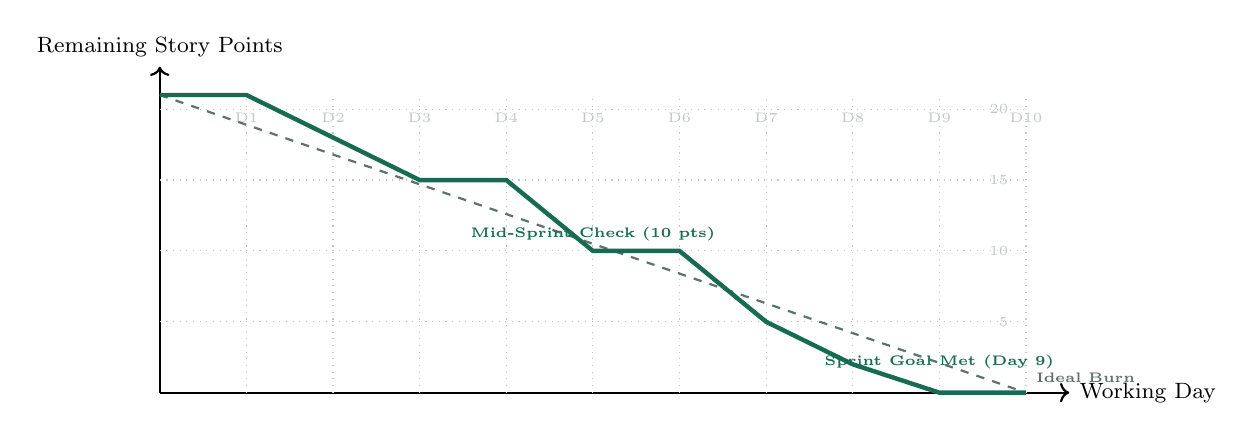
\begin{tikzpicture}
  \begin{scope}[xscale=1.1, yscale=0.18]
    \draw[->, thick] (0,0) -- (10.5,0) node[right, font=\footnotesize] {Working Day};
    \draw[->, thick] (0,0) -- (0,23) node[above, font=\footnotesize] {Remaining Story Points};
    
    \foreach \y in {5, 10, 15, 20}
      \draw[dotted, color=muted!40] (0,\y) -- (10,\y) node[left=0.1cm, font=\tiny] {\y};
    \foreach \x in {1, 2, 3, 4, 5, 6, 7, 8, 9, 10}
      \draw[dotted, color=muted!40] (\x,0) -- (\x,21) node[below=0.1cm, font=\tiny] {D\x};

    \draw[thick, dashed, color=muted] (0,21) -- (10,0) node[above right, font=\tiny\bfseries] {Ideal Burn};

    \draw[ultra thick, color=brand] 
      (0,21) -- (1,21) -- (2,18) -- (3,15) -- (4,15) -- (5,10) -- (6,10) -- (7,5) -- (8,2) -- (9,0) -- (10,0);
      
    \node[above, font=\tiny\bfseries, color=brand] at (5,10) {Mid-Sprint Check (10 pts)};
    \node[above, font=\tiny\bfseries, color=brand] at (9,1) {Sprint Goal Met (Day 9)};
  \end{scope}
\end{tikzpicture}
\caption{Sprint 1 Burndown Trajectory: 21 Committed Points}
\end{figure}

\section{Comprehensive Evaluation Protocol (D7 Preparation)}
\begin{itemize}[leftmargin=*]
  \item \textbf{Setting:} Booked controlled campus study room (quiet, ambient light, no external interruptions).
  \item \textbf{Cohort:} $N=6$ participants recruited from another COMP2300 project group.
  \item \textbf{UK GDPR Safeguards:} Zero sensitive personal data; zero collection of real financial records, utility bills, or household addresses. Standardized synthetic scenario cards used exclusively.
  \item \textbf{Tasks:}
    \begin{enumerate}
      \item T1: Home electricity logging (150 kWh) $\rightarrow$ verify contextual INR cost.
      \item T2: Assumptions audit $\rightarrow$ verify 0.716 kg/kWh factor, 2026 year, India scope.
      \item T3: Shift-work commute (15 km) marked as protected $\rightarrow$ verify action suppression.
      \item T4: Packaging logging (3 kg) $\rightarrow$ verify descriptive state without false credits.
      \item T5: Communal 500 kWh electricity bill $\rightarrow$ verify non-individual attribution.
    \end{enumerate}
  \item \textbf{Metrics:} Task Completion Rate, Time on Task ($\le 60$s for T1), Single Ease Question (1--7), System Usability Scale (SUS benchmark target $\ge 75/100$), and explain-back comprehension probes.
\end{itemize}

\end{document}
